%-------------------------------------------------------------------------------
%							PREAMBULE
%-------------------------------------------------------------------------------

\documentclass{beamer} 
% \documentclass[notes,handout]{beamer}   % Use this to print notes and disable animations

%%% Define colors and main theme-----
\usecolortheme{seahorse}

\usetheme[numbering=fraction,progressbar=head,block=fill,background=light,subsectionpage=progressbar]{metropolis} 

\useoutertheme{infolines}
\useoutertheme{smoothbars}

\definecolor{MyGray}{RGB}{188, 195, 196}
\setbeamercolor{date in head/foot}{fg=black,bg=MyGray}

\useinnertheme{rectangles}
%%-------------------------------------

\usepackage[fontsize=7.0]{scrextend} % Use this to force the fontsize


\usepackage{docmute} % To include multiple files

% \usepackage{tikz}
% \usetikzlibrary{positioning,shapes,arrows}
% \usetikzlibrary{babel}      % Utiliser ce Babel pour eviter les problemes avec les animations TIKX

\usepackage{etoolbox}
\newcommand{\zerodisplayskips}{%        %% To remove space after math box
  \setlength{\abovedisplayskip}{0pt}%
  \setlength{\belowdisplayskip}{0pt}%
  \setlength{\abovedisplayshortskip}{0pt}%
  \setlength{\belowdisplayshortskip}{0pt}}
% \appto{\normalsize}{\zerodisplayskips}
% \appto{\small}{\zerodisplayskips}
% \appto{\footnotesize}{\zerodisplayskips}

\usepackage{xcolor}
\usepackage{graphicx}
\usepackage{wrapfig}
\graphicspath{ {../report/Figures/} }
\usepackage[utf8]{inputenc}
\usepackage{amsmath,bm,mathtools}
\usepackage[font=normalsize]{caption}
\usepackage{subcaption}
% \captionsetup{labelformat=empty,labelsep=none}    % Pour retirer le terme figure des titres

\usepackage{marvosym} %% For smileys

\usepackage{multirow}
\newcommand{\tabhead}[1]{{\bfseries#1}}

\usepackage{cases}
\usepackage{siunitx}

\usepackage{mathdots}
% \usepackage{eulervm}    %% De beaux et droits symboles mathmatiques

\newcommand{\bvec}[1]{\bm{#1}}    %% Vecteur en gras
\newcommand{\myvec}[2]{\begin{pmatrix} #1  \\ #2 \end{pmatrix}}   %% vecteur 2d
\newcommand{\mymat}[4]{\begin{pmatrix} #1 & #2 \\ #3 & #4 \end{pmatrix}}  %% Matrice 2*2

\usepackage[backend=bibtex,style=authoryear,maxnames=2,natbib=true]{biblatex} % Use the bibtex backend with the authoryear citation style (which resembles APA)
\addbibresource{bibliography.bib} % The filename of the bibliography
\usepackage[autostyle=true]{csquotes} % Required to generate language-dependent quotes in the bibliography 
\renewcommand*{\bibfont}{\normalsize} % Pour reduire la taille des references

\usepackage{hyperref}
\usepackage{booktabs}

\usepackage{etoolbox}

\newcommand{\phifem}{$\phi$-FEM\kern1ex}


%-------------------------------------------------------------------------------
%							NEW COMMANDS
%-------------------------------------------------------------------------------
\newcommand{\R}{\mathbb{R}}
\newcommand{\N}{\ensuremath{\mathbb{N}}}
\renewcommand{\C}{\ensuremath{\mathbb{C}}}
\newcommand{\Z}{\ensuremath{\mathbb{Z}}}
\newcommand{\Q}{\ensuremath{\mathbb{Q}}}
\newcommand{\dd}{\partial}
\newcommand{\tmd}{{\hspace{0.17em}}d}
\newcommand{\dx}{{\hspace{0.17em}}dx}
\newcommand{\dt}{{\hspace{0.17em}}dt}
\newcommand{\dO}{{\hspace{0.17em}}d{\Omega}}
\newcommand{\dG}{{\hspace{0.17em}}d{\Gamma}}
\newcommand{\Th}{\mathcal{T}_h}
\DeclareMathOperator{\diam}{diam}


%-------------------------------------------------------------------------------
%							TITLE PAGE
%-------------------------------------------------------------------------------
\begin{document}


\title[PhiFEM]{\huge Simulation of soft tissues using innovative non-conforming Finite Elements Methods }

% \institute[University of Strasbourg]{\small \textbf{ \hspace*{0.1mm} Referent teacher} \hspace*{11mm} \textbf{Supervisors} \\ \footnotesize Christophe PRUD'HOMME \hspace*{4mm} Michel DUPREZ \\ \hspace*{38mm} Stephane COTIN}
\institute[University of Strasbourg]{University of Strasbourg}

% \institute[University of Strasbourg]{\normalsize \textbf{Enseignant} \\ Pr. Yannick PRIVAT}

\author[Desmond Roussel NZOYEM]{\normalsize \textbf{Author :} Desmond Roussel NZOYEM \\ \\ \small \textbf{Supervisors :} Michel DUPREZ, Stéphane COTIN \\ \textbf{Referent teacher :} Christophe PRUD'HOMME \\}

\date[\today]{M2 CSMI Project Course 2020/2021}

\begingroup  % A new group whose information is not canon. Just for this slide!
\setbeamertemplate{navigation symbols}{}
\setbeamertemplate{headline}{\vspace{0.5cm}%
  \hspace*{0.8cm}%
  \includegraphics[width=2.8cm]{LogoUnistra}
  \hfill\raisebox{.2cm}{\normalsize  }\hfill%
  \includegraphics[width=2.5cm]{LogoMimesis2.png}
  \hfill\raisebox{.2cm}{\normalsize  }\hfill%
  
\includegraphics[width=2.5cm]{LogoINRIA.png}
  \hfill\raisebox{.2cm}{\normalsize  }\hfill%
  
\includegraphics[width=2.5cm]{LogoCSMI}
  \hspace*{0.8cm}%
}
\begin{frame}[fragile]
\maketitle
\end{frame}
\endgroup


%-------------------------------------------------------------------------------
%							INCLUDE THE CHAPTERS
%-------------------------------------------------------------------------------

\begin{frame}
  \small
  \frametitle{Contents}
  \tableofcontents
\end{frame}


%-------------------------------------------------------------------------------
%							FIRST SECTION
%-------------------------------------------------------------------------------

\section{Project description}

\subsection{Environment and context}


\begin{frame}
    \frametitle{What is the environment?}

    \begin{enumerate}
        \item \textbf{Inria:} where \textcolor{teal}{\textbf{digital health}} is a main research topic\pause
        \item \textbf{MIMESIS:}
        \begin{itemize}
            \item real-time simulations for per-operative guidance
            \item data-driven simulation dedicated to patient-specific modeling
        \end{itemize}
    \end{enumerate}

    \begin{figure}
        \centering
        \includegraphics<2>[width=0.95\textwidth]{IntroPic.png}
        \caption{\only<2>{A few projects at MIMESI.}}
    \end{figure}
\end{frame}


\begin{frame}
    \frametitle{What are we trying to do?}

    The goal is to \textbf{develop a Finite Elements Method (FEM) adapted to computer-assisted surgery}. 
    
    \pause The FEM should be:
    \begin{itemize}
        \item quick; \pause
        \item precise; \pause
        \item patient-specific.
    \end{itemize}

\end{frame}


\subsection{Objectives}

\begin{frame}
    \frametitle{What is our goal?}

    \begin{itemize}
        \item \textbf{Main objective}: develop a \phifem technique for the dynamics of soft tissues. \pause
        \item \textbf{Intermediate objectives}: 
        \begin{enumerate}
            \item Understand the \phifem technique in question. \pause
            \item Reproduce the results from a preliminary study (the Poisson equation). \pause
            \item Develop a \phifem technique for the linear elasticity equation. \pause
            \item Use \phifem on body organ geometries.
        \end{enumerate}
        
    \end{itemize}
\end{frame}



% \begin{frame}
%     \frametitle{What is needed?}
%     \begin{itemize}
%         \item Computer Science 
%         \begin{enumerate}
%             \item Python
%             \item FEniCS
%             \item Docker
%             \item Sympy
%         \end{enumerate}
%         \item Mathematics
%         \begin{enumerate}
%             \item PDEs
%             \item Scientific computing
%             \item Numerical analysis
%         \end{enumerate}
%     \end{itemize}
% \end{frame}


%-------------------------------------------------------------------------------
%							SECOND SECTION
%-------------------------------------------------------------------------------

\section{Presentation of \phifem}

\subsection{The classic FEM framework}
\begin{frame}
    \frametitle{What is FEM?}

    \begin{figure}
        \centering
        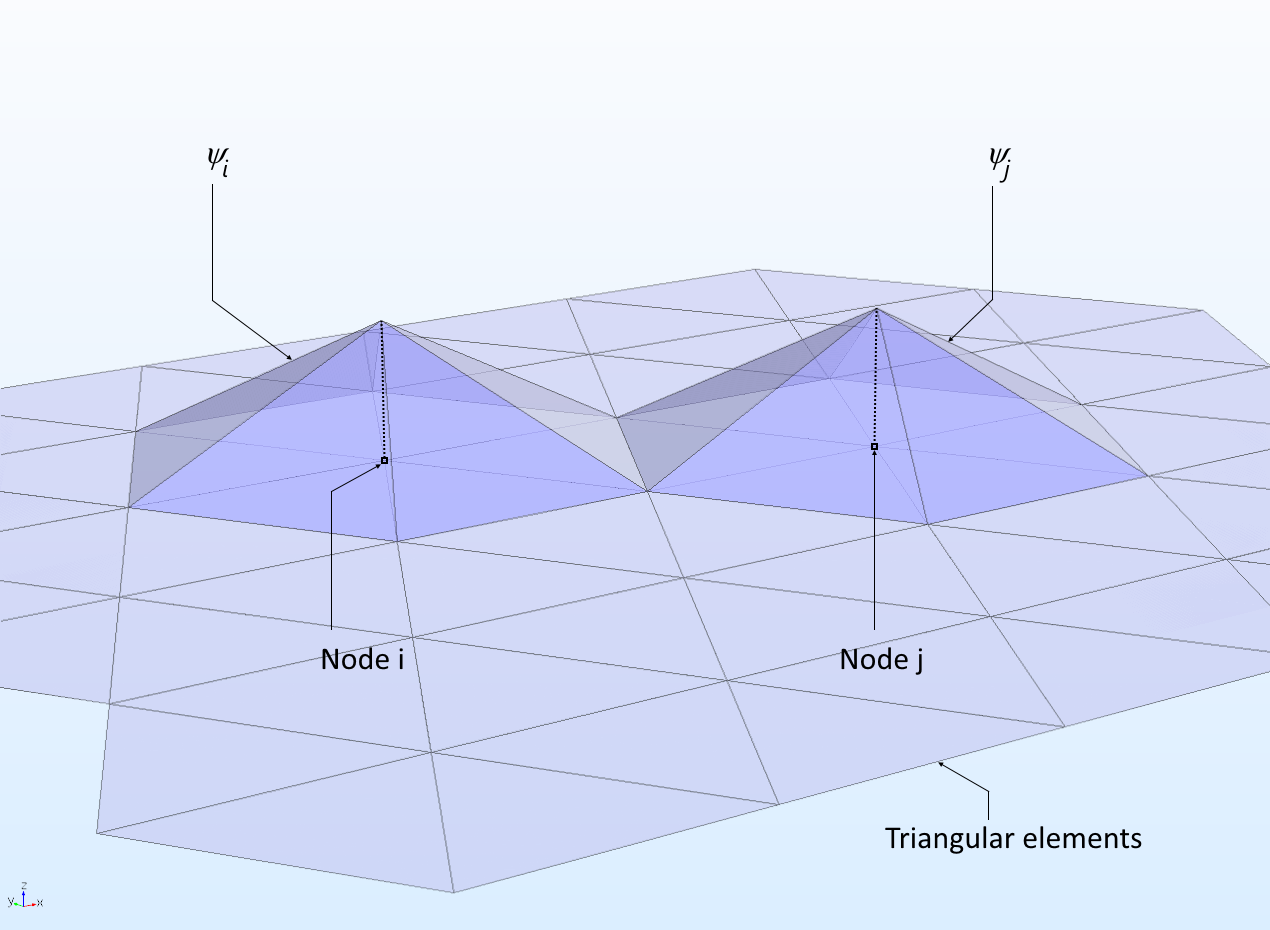
\includegraphics[width=0.8\textwidth]{FEM.png}
        \caption{Finite Elements Method (FEM) principle (\cite{cyclopedia}).}
    \end{figure}

\end{frame}



\subsection{Immersed boundary methods}


\begin{frame}

\frametitle{What are immersed boundary methods?}


\begin{wrapfigure}{r}{0.55\textwidth}
    \includegraphics<4>[width=0.9\linewidth]{XFEM.png} 
    \includegraphics<5>[width=0.8\linewidth]{CutFEM} 
    \includegraphics<6>[width=0.9\linewidth]{SBM} 
    \includegraphics<7>[width=0.9\linewidth]{PhiFEM} 
    \centering
    \only<4>{\caption{XFEM}}
    \only<5>{\caption{CutFEM}}
    \only<6>{\caption{SBM}}
    \only<7>{\caption{\phifem}}
    % \caption{\only<4>{XFEM}\only<5>{CutFEM}\only<6>{SBM}}
    \label{fig:immersed}
\end{wrapfigure}


Immersed boundary methods can handle:
\begin{itemize}
    \item complex geometries \pause
    \item non-body conforming grids \pause
    \item moving/evolving boundaries
\end{itemize}

\pause
Common examples are:
\begin{itemize}
    \item \textbf{XFEM} \parencite{de2018delamination}  \pause
    \item \textbf{CutFEM} \parencite{burman2015cutfem}\pause
    \item \textbf{SBM} \parencite{atallah2020analysis} \pause
    \item \textbf{\phifem}\parencite{Reference3}
\end{itemize}

\note{Les 3 premieres methodes demandes des integrations sur la forntiere. PhiFEM ne demande pas de telle integrations; la quadrature se passe sur la frontiere fictive.}

\end{frame}


\begin{frame}
    \frametitle{What is \phifem?}
The main ideas are (for Dirichlet boundary conditions): 
\begin{enumerate}
    \item \textbf{Define the domain using a level-set function $\phi$.}
    \item \textbf{Then make that function carry the solution: $u = \phi w + g$.}
\end{enumerate}
 
\begin{figure}
    \centering
    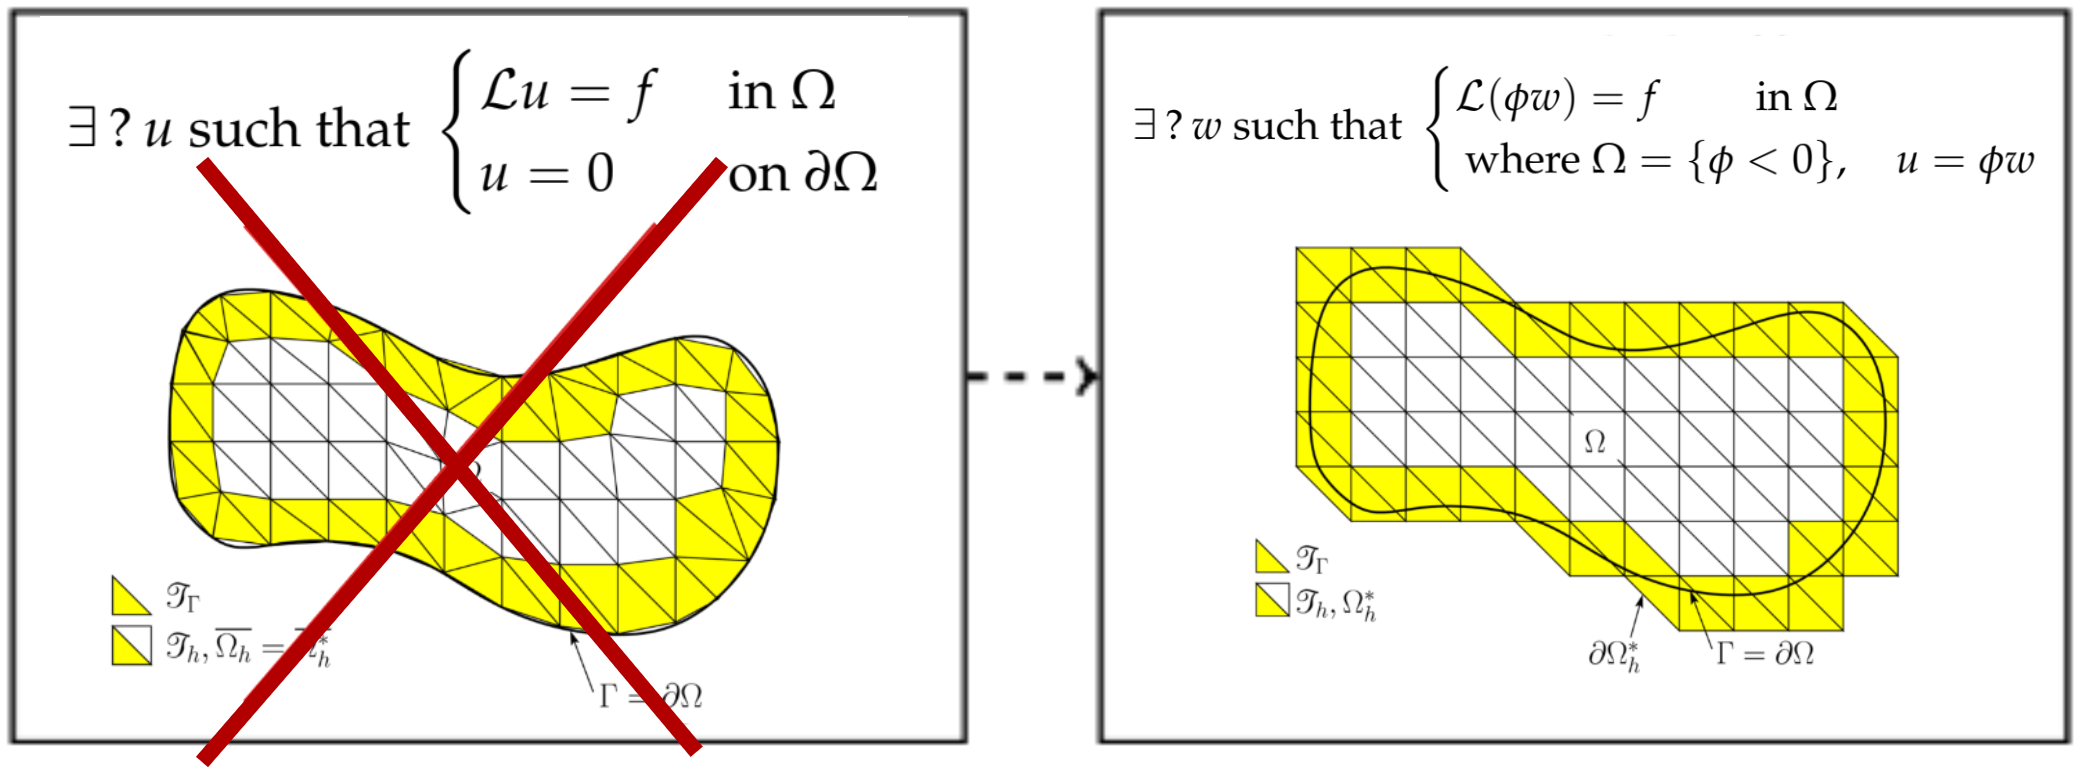
\includegraphics[width=0.95\textwidth]{ClassicToPhiFEM.png}
    \caption{From Classic FEM (on the left) to \phifem (on the right)}
\end{figure}
\end{frame}




%-------------------------------------------------------------------------------
%							THIRD SECTION
%-------------------------------------------------------------------------------

\section{Results}



% %% Template
% \begin{columns}[T]
%     \begin{column}{.48\textwidth}
%     \color{purple}\rule{\linewidth}{4pt}
%     Classic FEM \color{black}

%     \end{column}%
%     \hfill%
%     \begin{column}{.48\textwidth}
%     \color{orange}\rule{\linewidth}{4pt}
%     \phifem \color{black}

%     \end{column}%
% \end{columns}


\subsection{The Poisson problem}

\begin{frame}[t]
    \frametitle{Theoretical framework for the Poisson problem} The Poisson problem:
    \Large 
    \begin{align} 
        \begin{cases}
            -\Delta u = f  &\quad \text{in } \Omega \\
            u = 0  &\quad \text{on } \partial\Omega 
        \end{cases}
        \label{eq:poisson}
    \end{align}
    % \vspace*{0.1cm}
    \normalsize
    \pause
\begin{columns}[T] % align columns
    \begin{column}{.46\textwidth}
        \color{purple}\rule{\linewidth}{4pt}
        Classic FEM
        \color{black} \\ \footnotesize \vspace*{1pt}
        Find $u_h \in V_h^{(k)}$ such that
        \begin{align*}
            a_h(u_h,v_h)=l_h(v_h), \,\, \forall \, v_h \in V_h^{(k)},
        \end{align*}
        where
        \begin{align*}
            \notag
            a_h(u,v) & = \int_{\Omega_h} \nabla u \cdot \nabla v \\
            l_h(v) &= \int_{\Omega_h} fv \,.
            \label{eq:PoissonClassic}
        \end{align*}
        \hrule
    \end{column}%

    \hfill%
    
    \normalsize

    \pause
    \begin{column}{.50\textwidth}
        \color{orange}\rule{\linewidth}{4pt}
        \phifem 
        \color{black} \footnotesize (\cite{Reference3}) \\ \vspace*{1pt}
        First, write $u_h = \phi_h w_h$. Then find $w_h\in V_h^{(k)}$ such that
        \begin{equation*}
          a_h(w_h,v_h)=l_h(v_h)\mbox{ for all }v_h\in V_h^{(k)},
        \end{equation*}
        where
        \begin{equation*}
           a_h(w,v)=\displaystyle \int_{\Omega_h} \nabla (\phi_h w) \cdot \nabla (\phi_h v) -
           \textcolor{brown}{\int_{\partial \Omega_h} \frac{\partial}{\partial n} (\phi_h w) \phi_h
           v} + \textcolor{blue}{G_h (w, v)} 
        \end{equation*}	
           \[\displaystyle   l_h(v) = \int_{\Omega_h} f \phi_h v + \textcolor{red}{G_h^{rhs} (v)}. \]
    \end{column}%
\end{columns}
\pause
\footnotesize
\begin{align*} 
    \textcolor{blue}{G_h(w, v)} &: = \displaystyle\sigma h\sum_{E\in  \mathcal{F}_h^{\Gamma}} 
\int_E \left[ \frac{\partial}{\partial n}
   (\phi_h w) \right] \left[ \frac{\partial}{\partial n} ( \phi_hv)\right] + \sigma h^2 \sum_{T \in \Th^{\Gamma}} \int_T \Delta(\phi_h w) \Delta(\phi_h v)  
    \,, \\
    \textcolor{red}{G_h^{rhs} (v)} &: =\displaystyle- \sigma h^2\sum_{T \in\Th^{\Gamma}} \int_T f \Delta (\phi_h v)   
   \,.
\end{align*}

\end{frame}


\begin{frame}
    \frametitle{Numerical solution for the Poisson problem}

    \begin{columns}[T] % align columns
        \begin{column}{.48\textwidth}
        \color{purple}\rule{\linewidth}{4pt}
        Classic FEM \color{black}
        \begin{align*}
            \begin{cases}
            \Omega = \left\{ (x,y)\in\mathbb{R}^2: \left( x-\frac{1}{2} \right)^2 + \left( y-\frac{1}{2} \right)^2 < \frac{1}{8}  \right\} \\
            u(x,y)= -\left( \frac{1}{8} - \left( x-\frac{1}{2} \right)^2 - \left( y-\frac{1}{2} \right)^2 \right) \exp(x) \sin(2\pi y)\\
            f(x,y) = -\frac{\partial^2 u}{\partial x^2}(x,y) -\frac{\partial^2 u}{\partial y^2}(x,y)
            \end{cases}
        \end{align*}
        
        \end{column}%
        \hfill%
        \begin{column}{.48\textwidth}
        \color{orange}\rule{\linewidth}{4pt}
        \phifem \color{black}
        \begin{align*}
            \begin{cases}
            \mathcal{O} = [0,1]\times[0,1] \\
            \phi(x,y) = -\frac{1}{8} + \left( x-\frac{1}{2} \right)^2 + \left( y-\frac{1}{2} \right)^2 \\
            u(x,y)=\phi(x,y) \times \exp(x) \times \sin(2\pi y) \\
            f(x,y) = -\frac{\partial^2 u}{\partial x^2}(x,y) -\frac{\partial^2 u}{\partial y^2}(x,y) \\
            \sigma = 20
            \end{cases}
        \end{align*}
        
        \end{column}%
    \end{columns}

    \pause

    \begin{columns}
        \begin{column}{0.48\textwidth}
            \centering
            \begin{figure}            
            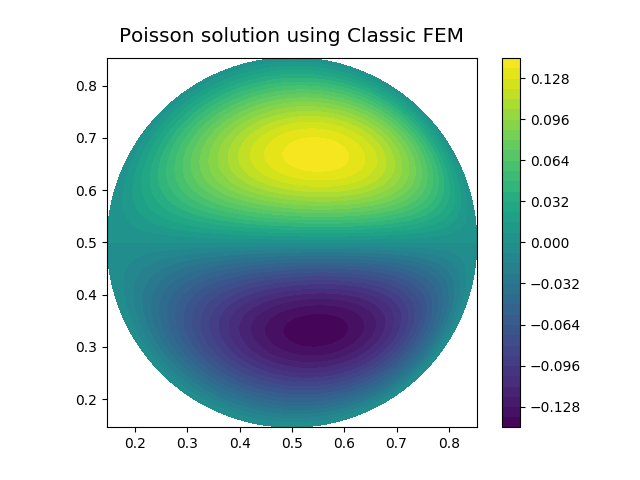
\includegraphics[width=0.95\textwidth]{ClassicSol2.png}
            \caption{Classic FEM ($39642$ cells)}
            \end{figure}
        \end{column}
        \begin{column}{0.48\textwidth}
            \centering
            \begin{figure}            
            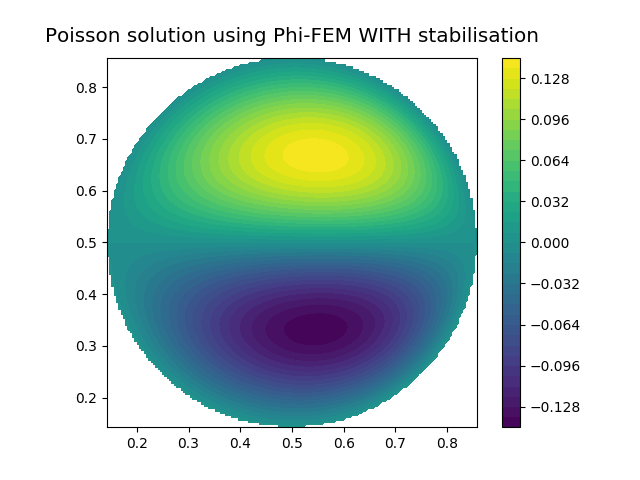
\includegraphics[width=0.95\textwidth]{StabSol.png}
            \caption{\phifem ($39936$ cells)}
            \end{figure}
        \end{column}
    \end{columns}

    \note{Remarque sur la non-smoothness de la solution sur les bords. C'est parcequ'un disque c'est facilement maillable!}

\end{frame}

\begin{frame}
    \frametitle{Convergence study for the Poisson Problem}

\begin{columns}
    \begin{column}{0.48\textwidth}
        \centering
        \begin{figure}            
        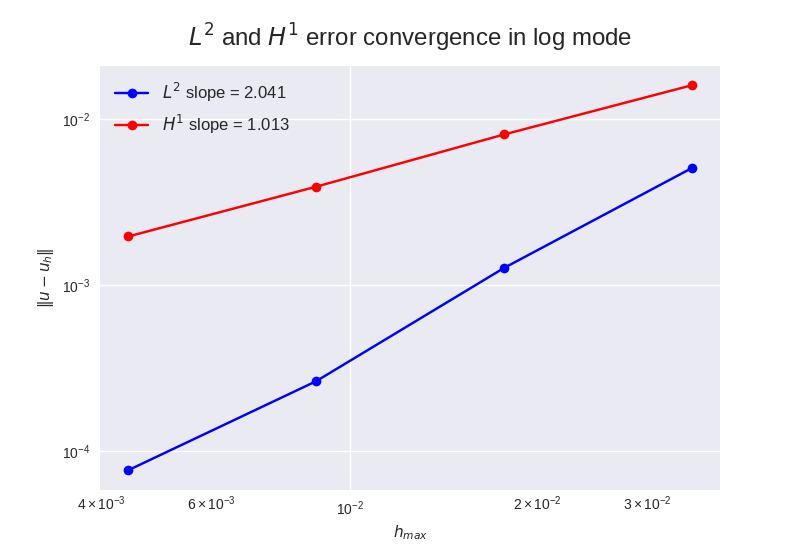
\includegraphics[width=0.95\textwidth]{ClassicCvgStudy2.png}
        \caption{Classic FEM}
        \end{figure}
    \end{column}
    \begin{column}{0.48\textwidth}
        \centering
        \begin{figure}            
        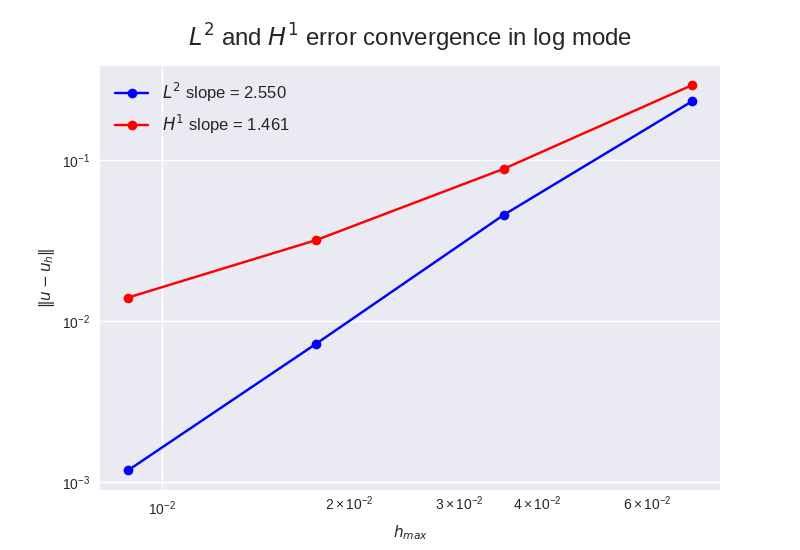
\includegraphics[width=0.95\textwidth]{StabCvgStudy.png}
        \caption{\phifem}
        \end{figure}
    \end{column}
\end{columns}

\begin{table}[h!]
    \centering
    \begin{tabular}{c| l| c| c}
        \toprule
        \tabhead{Problem} & \tabhead{Technique} & \tabhead{$L^2$ slope} & \tabhead{$H^1$ slope} \\
        \midrule
        \multirow{2}{4em}{Poisson} & Classic FEM & 2.041 & 1.013 \\
         & \phifem & 2.550 & 1.461 \\
        \bottomrule
    \end{tabular}
    \caption{Convergence rates.}
  \end{table}

\end{frame}






\subsection{The elasticity equation}

\begin{frame}[t]
    \frametitle{Theoretical framework for the elasticity equation} The elasticity equation: \large
    \begin{align}
        \begin{cases}
        \nabla \cdot \sigma(u) + f = 0 &\quad \text{in } \Omega\\   
        \sigma(u) = \lambda(\nabla \cdot u) \mathcal{I} + \mu (\nabla u + \nabla u^T)  &\quad \text{in } \Omega\\
        u = g &\quad \text{on } \partial\Omega
        \end{cases}
        \label{eq:elasticity}
    \end{align}
    % \vspace*{0.1cm}
    \normalsize

    \pause

    \note{Rappler qu'il s'agit d'une formulation variationnelle dans l'espace H1, et non l'approximation éléments finis. Ce qui fait qu'on peut enlever le subscript h. }

\begin{columns}[T] % align columns
    \begin{column}{.44\textwidth}
        \color{purple}\rule{\linewidth}{4pt}
        Classic FEM
        \color{black} \\ \footnotesize
        First $V=\left[H_0^1(\Omega)\right]^d$, and $\gamma G = g$. Then find $u \in G + V $ such that
        \begin{align*}
         a(u,v)=l(v), \quad \forall v \in V
        \end{align*}
        where $a$ and $l$ are defined as 
        $$
        a(u,v) = \int_{\Omega} \sigma (u) : \varepsilon (v)
        $$
        and
        $$
        l(v) = \int_{\Omega} f\cdot v
        $$
    \hrule
    \end{column}%

    \hfill%
    \pause
    
    \normalsize
    \begin{column}{.52\textwidth}
        \color{orange}\rule{\linewidth}{4pt}
        \phifem 
        \color{black} \\ \footnotesize
        First, $u_h = \phi w + g$. Then find $w \in V$ such that:
        \begin{align*}
            a(w,v)=l(v), \quad \forall v \in V
        \end{align*}
        where $a$ and $l$ are defined as 
        $$
        a(w,v) = \int_{\Omega} \sigma(\phi w) : \varepsilon(\phi v) - \textcolor{brown}{\int_{\partial\Omega} (\sigma(\phi w) \cdot n) \cdot (\phi v)} + \textcolor{blue}{G(w,v)}
        $$
        and
        $$
        l(v) = \int_{\Omega} f \cdot (\phi v) + \textcolor{teal}{\int_{\partial\Omega} (\sigma(g) \cdot n) \cdot (\phi v)} - \textcolor{magenta}{\int_{\Omega} \sigma(g) : \varepsilon(\phi v)} + \textcolor{red}{G_{rhs}(v)}
        $$        
    \end{column}%
\end{columns}
\pause
\footnotesize
$$
\textcolor{blue}{G(w,v)} = \sigma_{pen} h^2 \sum_{E \in \mathcal{T}_h^{\Gamma}} \int_{E} \left(\nabla \cdot \sigma(\phi w)\right) \cdot \left( \nabla \cdot \sigma(\phi v)\right) + \sigma_{pen} h \sum_{F \in \mathcal{F}_h^{\Gamma}} \int_{F} \left[\sigma(\phi w) \cdot n \right] \cdot \left[ \sigma(\phi v) \cdot n \right] 
$$ 

$$
\textcolor{red}{G_{rhs}(v)} = - \sigma_{pen} h^2 \sum_{E \in \mathcal{T}_h^{\Gamma}} \int_{E} \left( f + \nabla \cdot \sigma(g) \right) \cdot \left( \nabla \cdot \sigma(\phi v)\right) - \sigma_{pen} h \sum_{F \in \mathcal{F}_h^{\Gamma}} \int_{F} \left[\sigma(g) \cdot n \right] \cdot \left[ \sigma(\phi v) \cdot n \right]
$$


\end{frame}

\small

\begin{frame}
    \frametitle{Numerical solution for the elasticity equation}

    \begin{columns}[T] % align columns
        \begin{column}{.48\textwidth}
        \color{purple}\rule{\linewidth}{4pt}
        Classic FEM \color{black}
        \begin{align*}
            \begin{cases}
            \Omega = \left\{ (x,y)\in\mathbb{R}^2: \left( x-\frac{1}{2} \right)^2 + \left( y-\frac{1}{2} \right)^2 < \frac{1}{8}  \right\} \\
            u(x,y)= \begin{pmatrix}
                2x + \sin(x)\exp(y) \\ \frac{x}{2} + \cos(x) - 1
            \end{pmatrix}  \\
            f(x,y) = -\nabla \cdot \sigma(u(x,y)) \\
            g(x,y) = u(x,y)
            \end{cases}
        \end{align*}
        
        \note{Signaler que g n'est pas egale à u sur les bords, ceci afin d'introduire une perturbation qui sera résolue par les termes de penalisation.}

        \end{column}%
        \hfill%
        \begin{column}{.48\textwidth}
        \color{orange}\rule{\linewidth}{4pt}
        \phifem \color{black}
        \begin{align*}
            \begin{cases}
            \mathcal{O} = [0,1]\times[0,1] \\
            \phi(x,y) = -\frac{1}{8} + \left( x-\frac{1}{2} \right)^2 + \left( y-\frac{1}{2} \right)^2 \\
            u(x,y)= \begin{pmatrix}
                2x + \sin(x)\exp(y) \\ \frac{x}{2} + \cos(x) - 1
            \end{pmatrix}  \\
            f(x,y) = -\nabla \cdot \sigma(u(x,y)) \\
            g(x,y) = u(x,y) + \textcolor{blue}{\phi(x,y) \begin{pmatrix}
               \sin(x) \\ \exp(y)
            \end{pmatrix}} \\
            \sigma_{pen} = 20
            \end{cases}
        \end{align*}
        

        \end{column}%
    \end{columns}

    \pause

    \begin{columns}
        \begin{column}{0.4\textwidth}
            \centering
            \begin{figure}            
            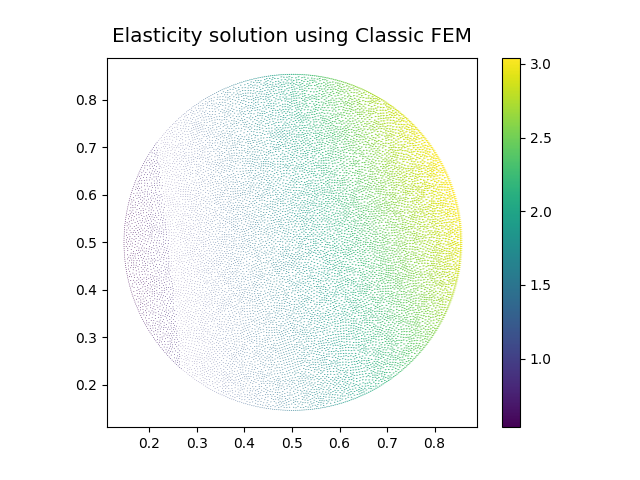
\includegraphics[width=0.95\textwidth]{ClassicElasSol.png}
            \caption{Classic FEM}
            \end{figure}
        \end{column}
        \begin{column}{0.4\textwidth}
            \centering
            \begin{figure}            
            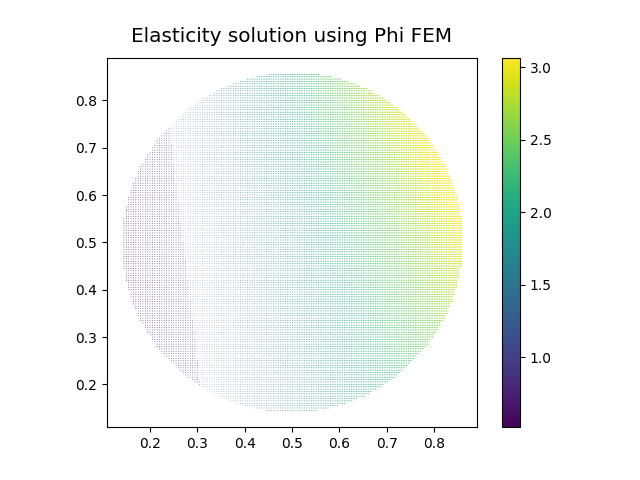
\includegraphics[width=0.95\textwidth]{StabElasSol.png}
            \caption{\phifem}
            \end{figure}
        \end{column}
    \end{columns}

\end{frame}

\begin{frame}
    \frametitle{Numerical solution for the elasticity equation (cont.)}

    \begin{figure}[H]
        % \centering
        \begin{subfigure}{0.2\textwidth}
            % \centering
            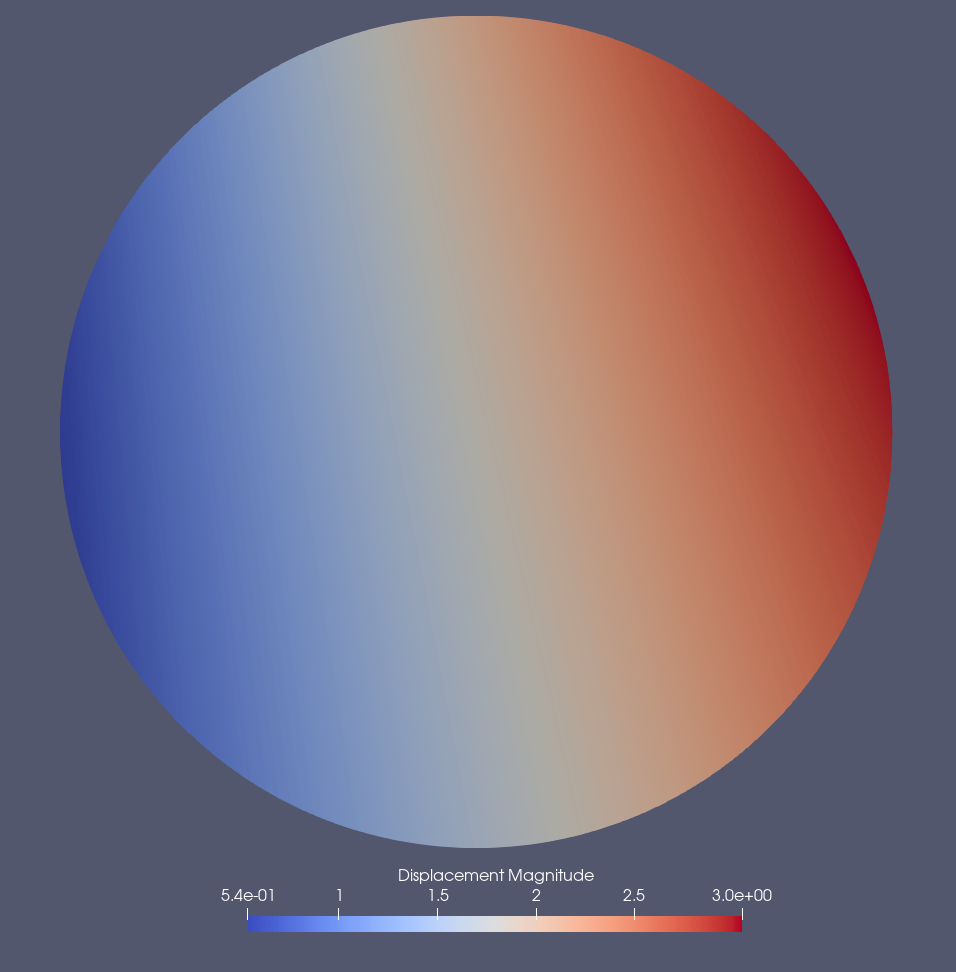
\includegraphics[width=\textwidth]{ClassicElasPara1.png}
          \caption{Classic FEM}
        \end{subfigure}
        \begin{subfigure}{0.21\textwidth}
            % \centering
            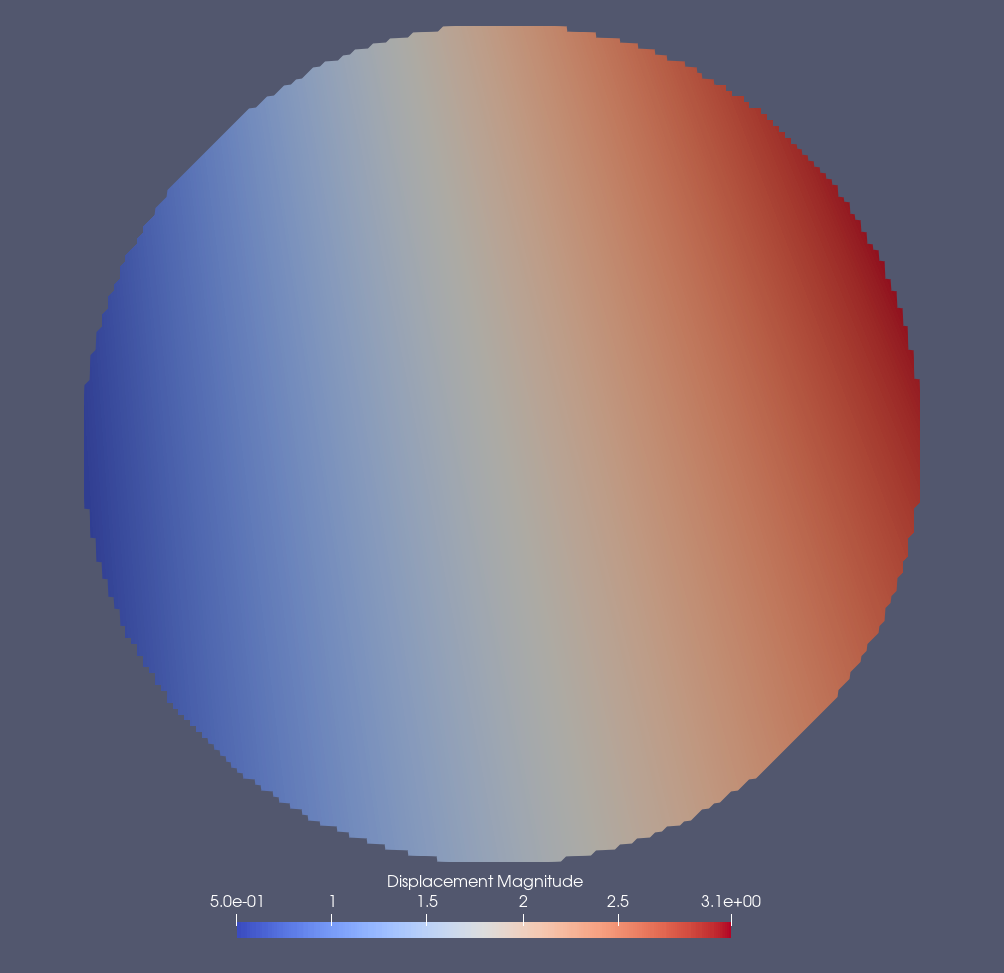
\includegraphics[width=\textwidth]{StabElasPara1.png}
          \caption{\phifem}
        \end{subfigure}
        \caption{Solution (deformation) magnitude in Paraview.}
    \end{figure}
    
    \zerodisplayskips
    \begin{figure}[H]
        % \centering
        \begin{subfigure}{0.2\textwidth}
            % \centering
            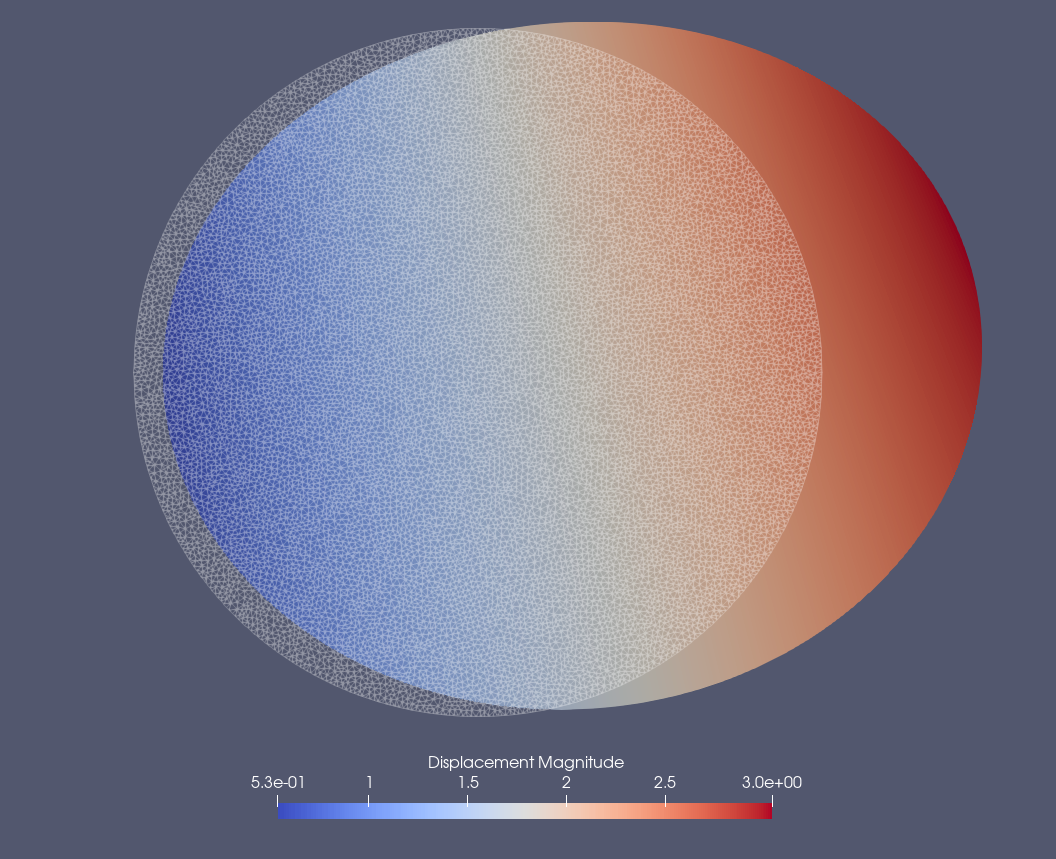
\includegraphics[width=\textwidth]{ClassicElasPara2.png}
          \caption{Classic FEM}
        \end{subfigure}
        \begin{subfigure}{0.21\textwidth}
            % \centering
            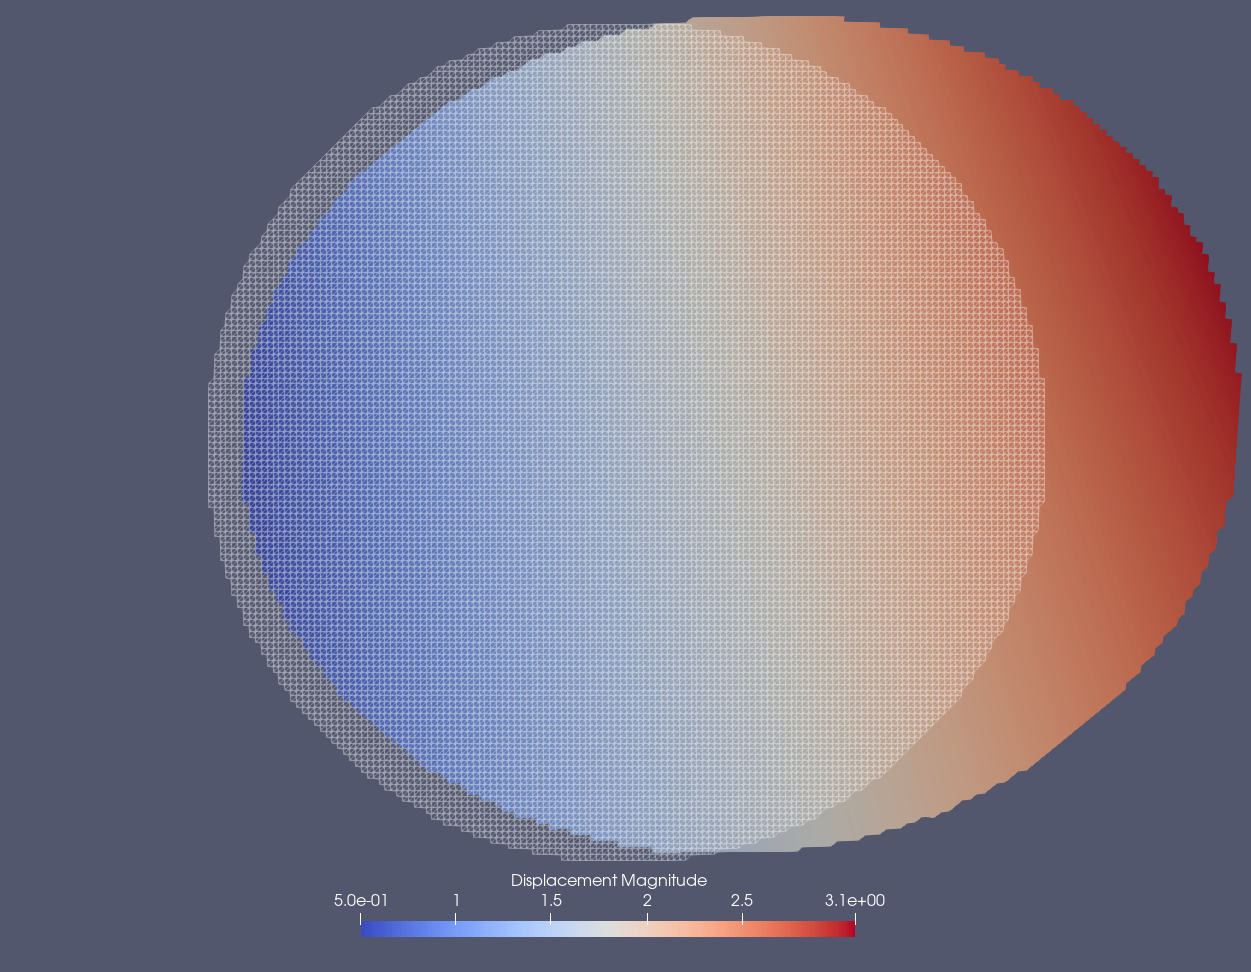
\includegraphics[width=\textwidth]{StabElasPara2.png}
          \caption{\phifem}
        \end{subfigure}
        \caption{Solution warped by vector in Paraview.}
    \end{figure}
    
    
\end{frame}

\begin{frame}
    \frametitle{Convergence study for the elasticity equation}

\begin{columns}
    \begin{column}{0.48\textwidth}
        \centering
        \begin{figure}            
        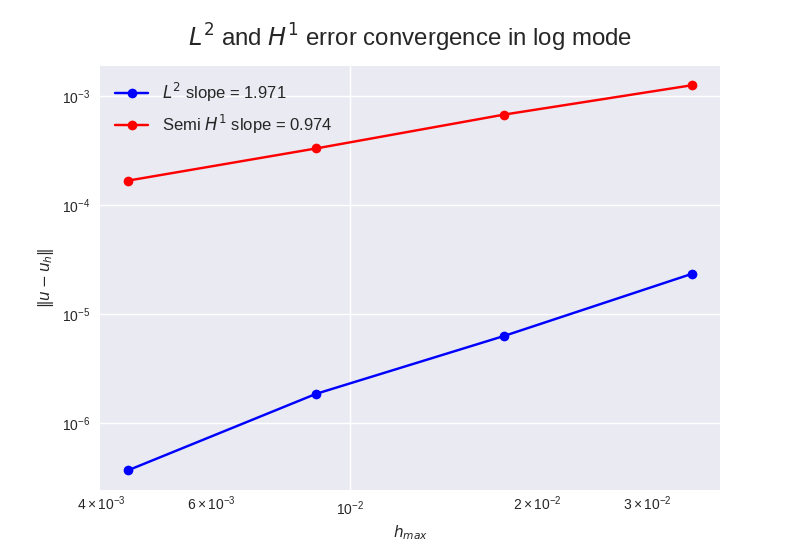
\includegraphics[width=0.95\textwidth]{ClassicElasCvg.png}
        \caption{Classic FEM}
        \end{figure}
    \end{column}
    \begin{column}{0.48\textwidth}
        \centering
        \begin{figure}            
        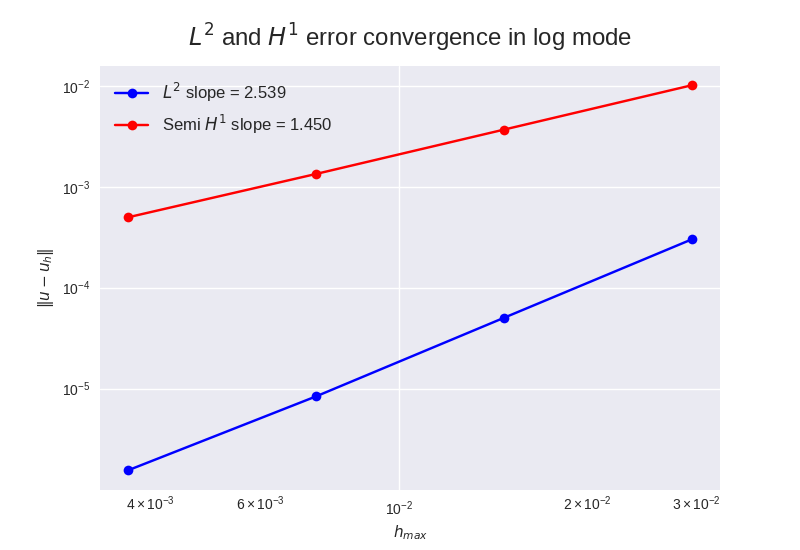
\includegraphics[width=0.95\textwidth]{StabElasCvg.png}
        \caption{\phifem}
        \end{figure}
    \end{column}
\end{columns}

\note{Rappeller qu'il s'agit des semi-normes H1.}

\begin{table}[h!]
    \centering
    \begin{tabular}{c| l| c| c}
        \toprule
        \tabhead{Problem} & \tabhead{Technique} & \tabhead{$L^2$ slope} & \tabhead{$H^1$ slope} \\
        \midrule
        \multirow{2}{4em}{Elasticity} & Classic FEM & 1.971 & 0.974 \\
         & \phifem & 2.539 & 1.450 \\
        \bottomrule
    \end{tabular}
    \caption{Convergence rates.}
\end{table}

  
\end{frame}



%-------------------------------------------------------------------------------
%							FOURTH SECTION
%-------------------------------------------------------------------------------


\section{Project summary}

\subsection{Work done}

\begin{frame}
    \frametitle{What has been done?}
    Based on the objectives, the deadlines, and the time estimates we set early in the project:
    \begin{itemize}
        \item[\checkmark] \textbf{Understanding \phifem}: November 3rd, 2020 : \alert{10 hours}  \pause
        \item[\checkmark] \textbf{Implementing the Poisson equation}: November 10, 2020 : \alert{50 hours} \pause
        \item[\checkmark] \textbf{Implementing the elasticity equation}: January 19, 2021 : \alert{30 hours}  \pause
        \item[$\times$] \textbf{Simulations on organ geometries}: January 19, 2021 : \alert{00 hours} \pause
    \end{itemize}
    
    Possible explorations:
    \begin{itemize}
        \item Test the technique on complex geometries. \pause
        \item Benchmark the technique for speed efficiency. \pause
        \item Deploy the numerical implementation into the SOFA software. \pause
        \item Implement the Neuman case (\cite{Reference4}).
    \end{itemize}

\end{frame}



\subsection{Delivered documents}
\begin{frame}
    \frametitle{What did I deliver?}
    As promised:
    \begin{enumerate}
        \item A typewritten report \pause
        \item A Python code base
    \end{enumerate}
    All are available on \href{https://github.com/master-csmi/2020-m2-mimesis}{this GitHub repository}: \url{https://github.com/master-csmi/2020-m2-mimesis} 
\end{frame}


% 
%-------------------------------------------------------------------------------
%							FITH SECTION
%-------------------------------------------------------------------------------



%% Form this point on, use the dark theme
\metroset{background=dark}

% %-------------------------------------------------------------------------------
% %							THE BIBLIOGRAPHY
% %-------------------------------------------------------------------------------
\appendix   % Pour retirer les references de la bare de navigation
% \vspace*{0.5mm}
\printbibliography


% %-------------------------------------------------------------------------------
% %							THANK YOU NOTE
% %-------------------------------------------------------------------------------

% \begingroup
% \section{Thx for your kind attention \Large \Smiley{} ! \\ Questions ?}
% \begin{frame}[standout]
\begin{frame}
  \Large
  \centering
  Thank you for your kind attention \Large \Smiley{} ! \\
  \centering
  Questions ?
\end{frame}

% \endgroup


\end{document}
